\chapter{Appendix}

\section{Variations for signal strength visualization over time}
\label{appendix_signal_strength}

This section contains various visualizations for different users' scanned access
points over time. On the x axis we have the time frame, while on the y axis we
have the signal strength for the identified access points. The legend presents
only the top $10$ predominant access points (which have appeared the most
during scans), however the plot displays all access points. The figures are
Fig.~\ref{user_6_cross_1d}, Fig.\ref{user_6_star_1d},
Fig.~\ref{user_6_cross_line_1d}, Fig.\ref{user_6_o_line_1d}.

\begin{figure}[!h]
\centering
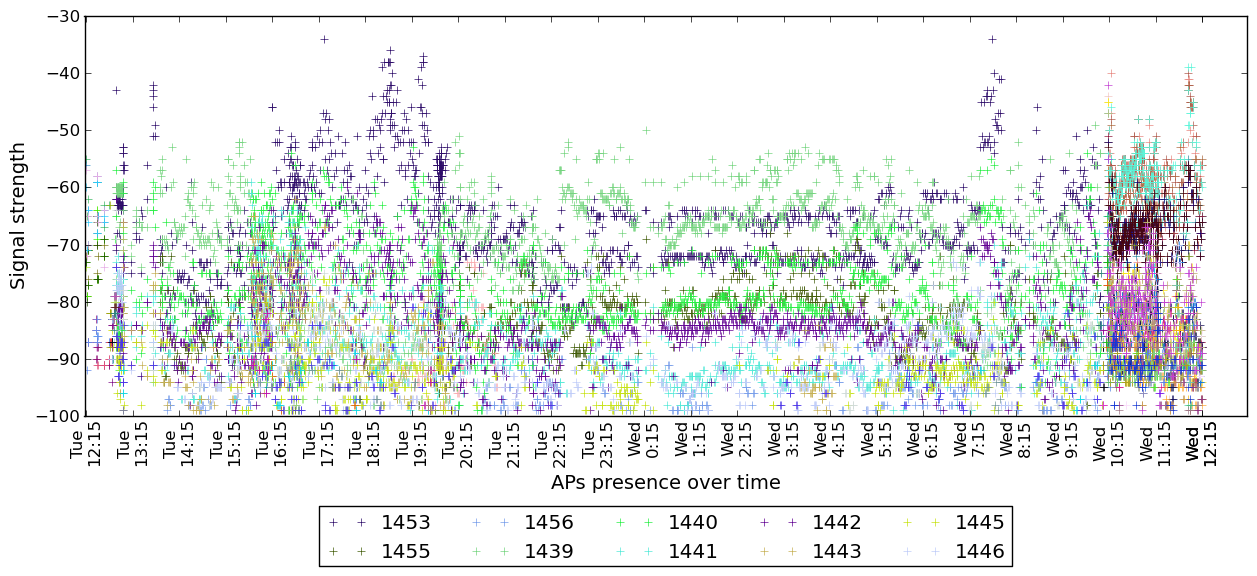
\includegraphics[height =
0.45\textwidth]{figures/cros_user_6_sorted_1days_plot.png}
\caption{Example of the APs registered for userX throughout one day with
``+'' markers}
\label{user_6_cross_1d}
\end{figure}

\begin{figure}[!h]
\centering
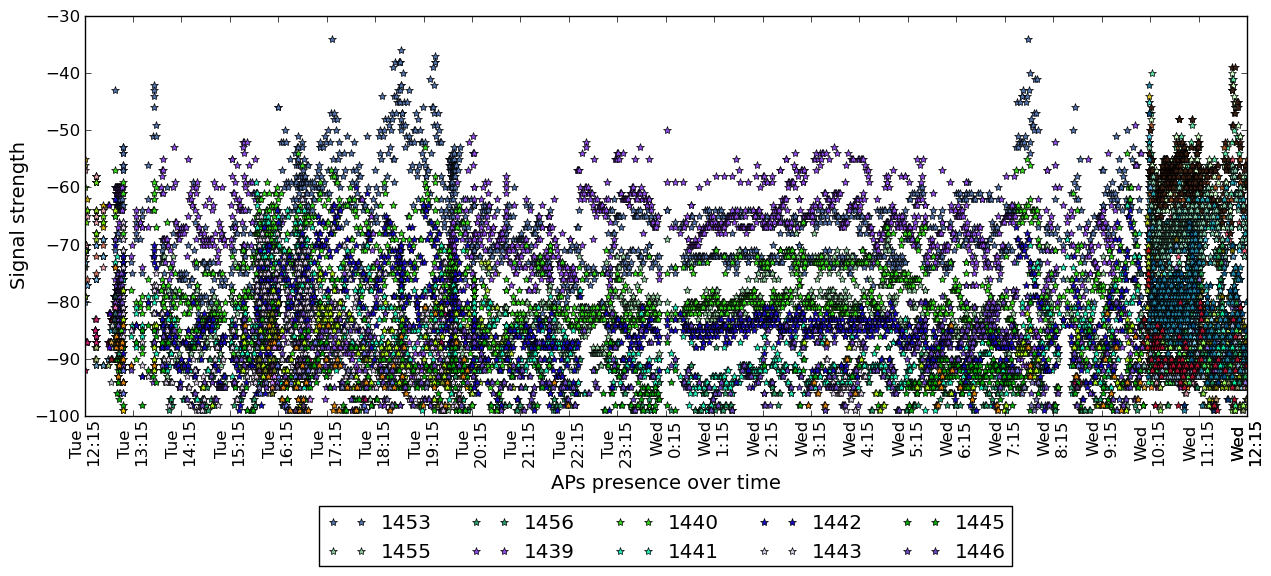
\includegraphics[height =
0.45\textwidth]{figures/star_user_6_sorted_1days_plot.png}
\caption{Example of the APs registered for userX throughout one day with
``*'' markers}
\label{user_6_star_1d}
\end{figure}

\begin{figure}[!h]
\centering
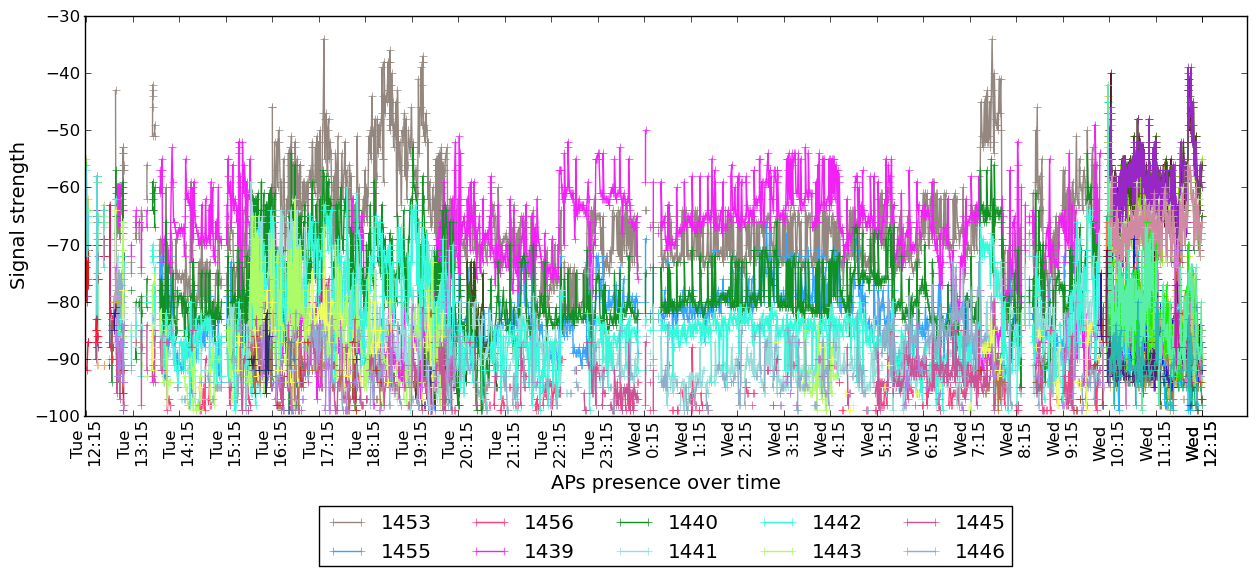
\includegraphics[height =
0.45\textwidth]{figures/cros_line_user_6_sorted_1days_plot.png}
\caption{Example of the APs registered for userX throughout one day with
``+'' and line markers}
\label{user_6_cross_line_1d}
\end{figure}

\begin{figure}[!h]
\centering
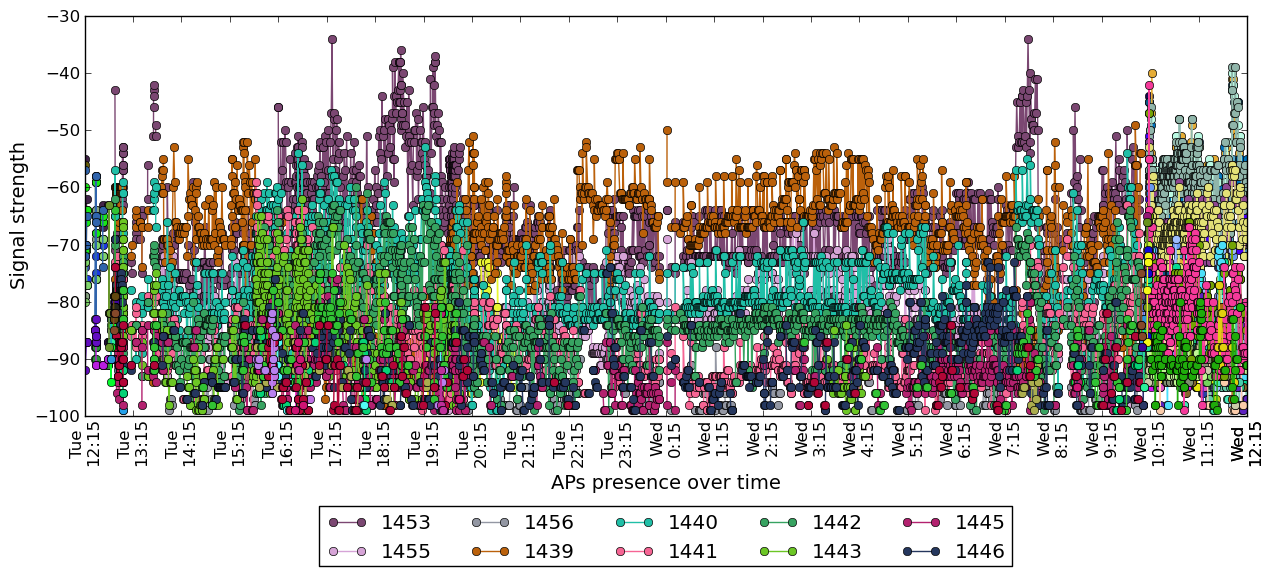
\includegraphics[height =
0.45\textwidth]{figures/o_line_user_6_sorted_1days_plot.png}
\caption{Example of the APs registered for an user throughout one day with
``o'' and line markers}
\label{user_6_o_line_1d}
\end{figure}

\section{Sample density for APs identified for a user}
\label{appendix_sample_density}

This section contains the visualization for the signal strength of different APs
that have been identified as being associated to a user throughout a period of
$1$ day (Fig.~\ref{rssi_6_2nd_day}) as well as the sample density visualizations
for the top various APs that were scanned throughout this time
(Fig.~\ref{samples_6_2nd_day_1},Fig.~\ref{samples_6_2nd_day_2},Fig.~\ref{samples_6_2nd_day_3}).

\begin{figure}[!h]
\centering
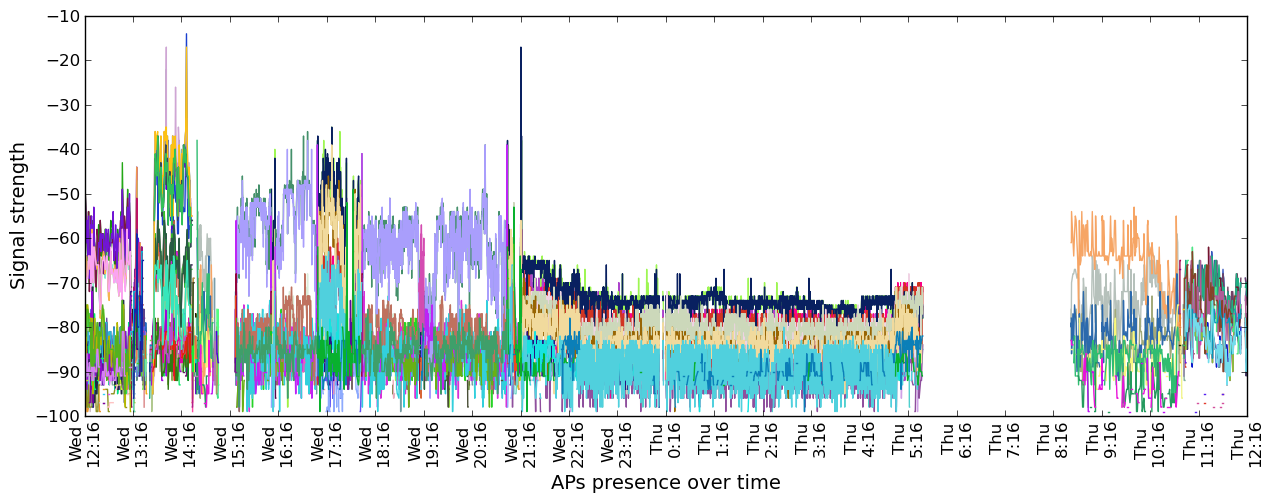
\includegraphics[width =\textwidth]{figures/combinations/user_6_sorted_1days_plot_croped.png}
\caption{Example of the APs registered for userZ throughout 1 day}
\label{rssi_6_2nd_day}
\end{figure}

\begin{figure}[!h]
\centering
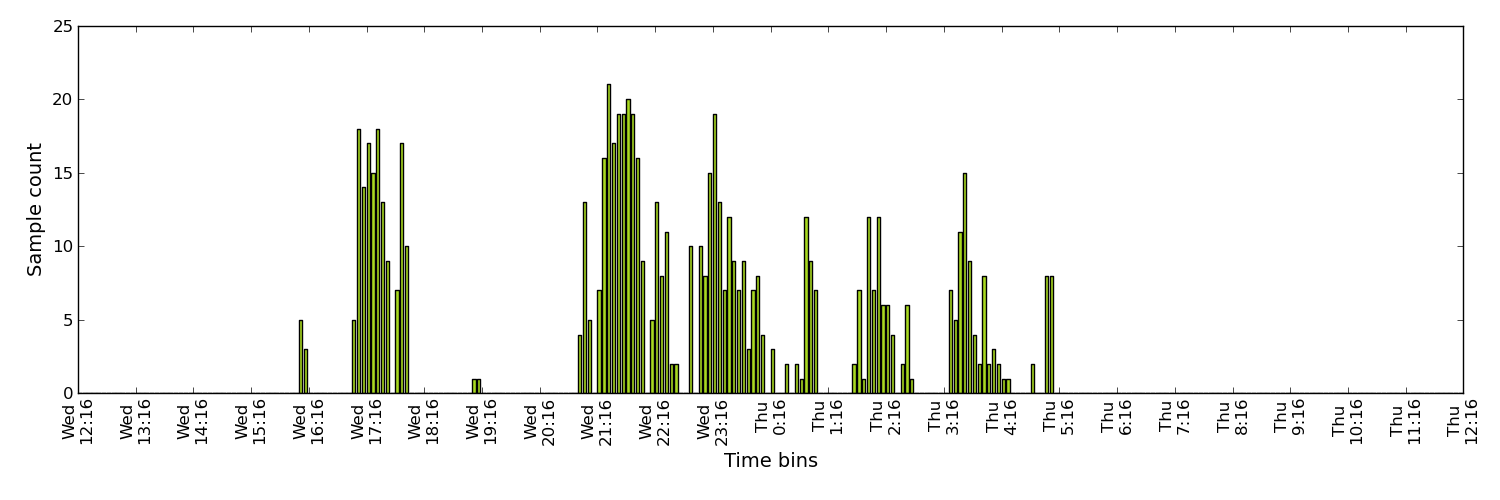
\includegraphics[width =\textwidth]{figures/combinations/ap_15188_histo.png}
\caption{Sample density of AP 15188 for userZ}
\label{samples_6_2nd_day_1}
\end{figure}

\begin{figure}[!h]
\centering
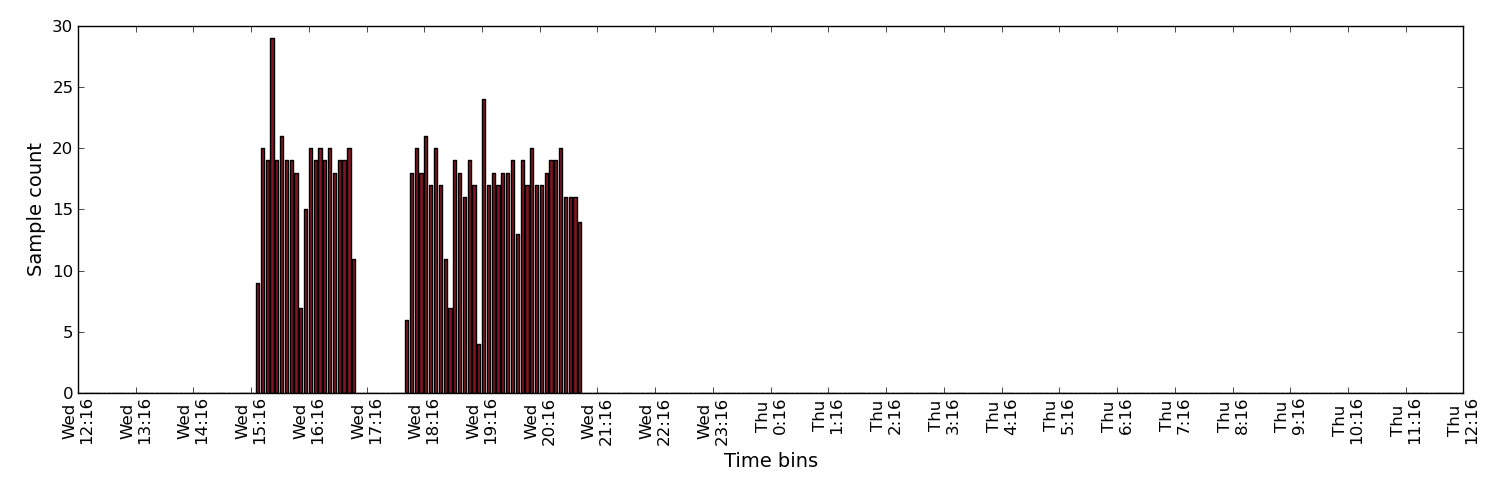
\includegraphics[width =\textwidth]{figures/combinations/ap_15190_histo.png}
\caption{Sample density of AP 15190 for userZ}
\label{samples_6_2nd_day_2}
\end{figure}

\begin{figure}[!h]
\centering
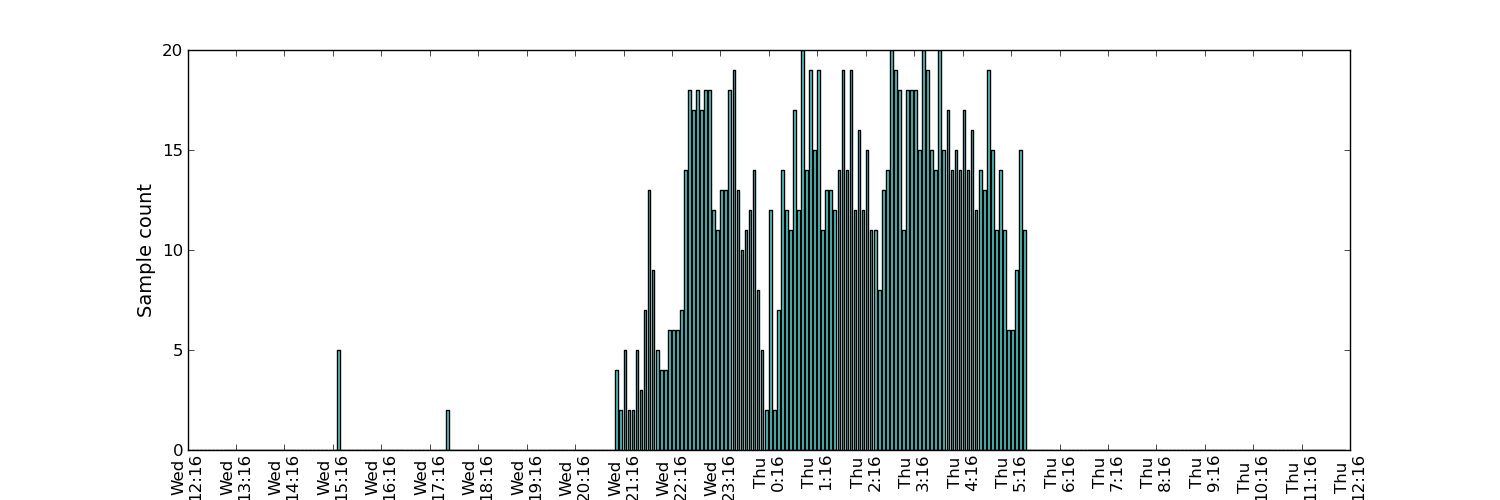
\includegraphics[width =\textwidth]{figures/combinations/ap_3144_histo.png}
\caption{Sample density of AP 3144 for userZ}
\label{samples_6_2nd_day_3}
\end{figure}

\subsection{Average signal strength for APs identified for a user}
\label{appendix_avg_signal}

This section contains the visualization for the signal strength of APs 15188
(Fig.~\ref{avg_6_2nd_day_1}), 15190 (Fig.~\ref{avg_6_2nd_day_2}) and 3144
(Fig.~\ref{avg_6_2nd_day_3}) calculated for $5$ minutes time bins over the
course of one day from the data gathered for userZ.

\begin{figure}[!h]
\centering
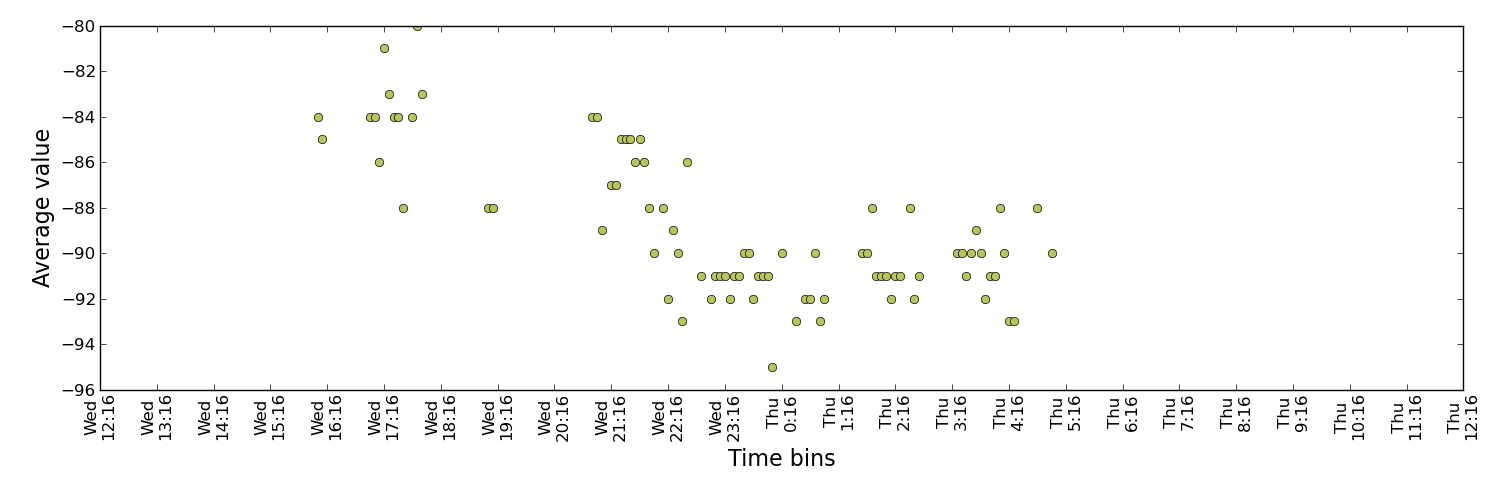
\includegraphics[width =\textwidth]{figures/combinations/user_6_sorted_1days_plot_15188_avg_sig.png}
\caption{Sample density of AP 15188 for userZ}
\label{avg_6_2nd_day_1}
\end{figure}

\begin{figure}[!h]
\centering
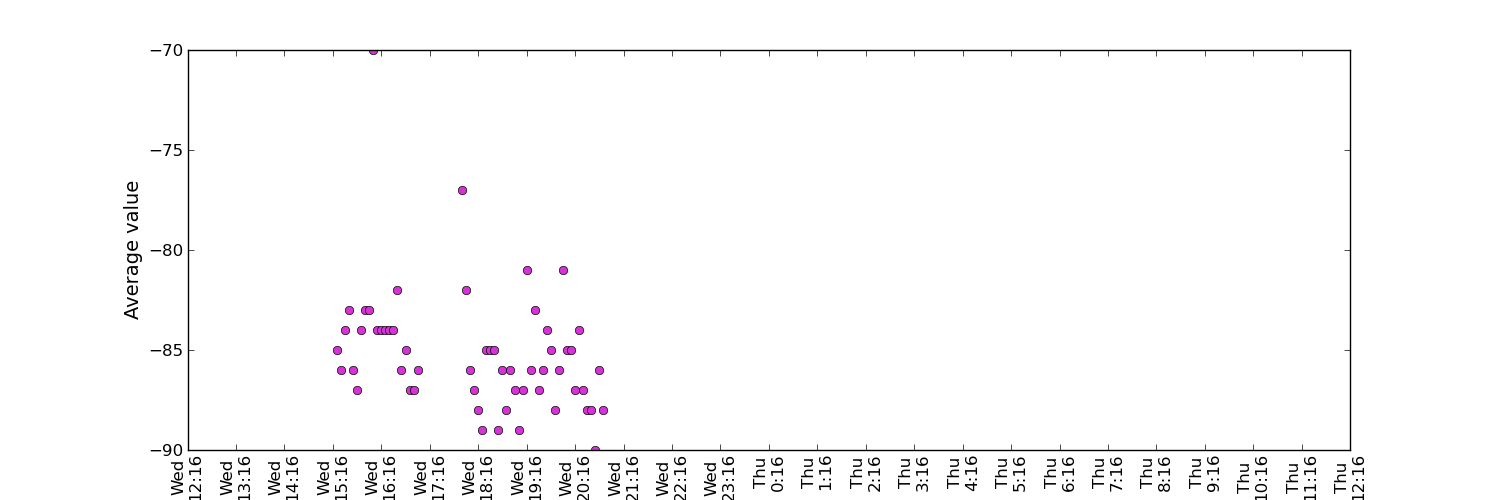
\includegraphics[width =\textwidth]{figures/combinations/user_6_sorted_1days_plot_15190_avg_sig.png}
\caption{Sample density of AP 15190 for userZ}
\label{avg_6_2nd_day_2}
\end{figure}

\begin{figure}[!h]
\centering
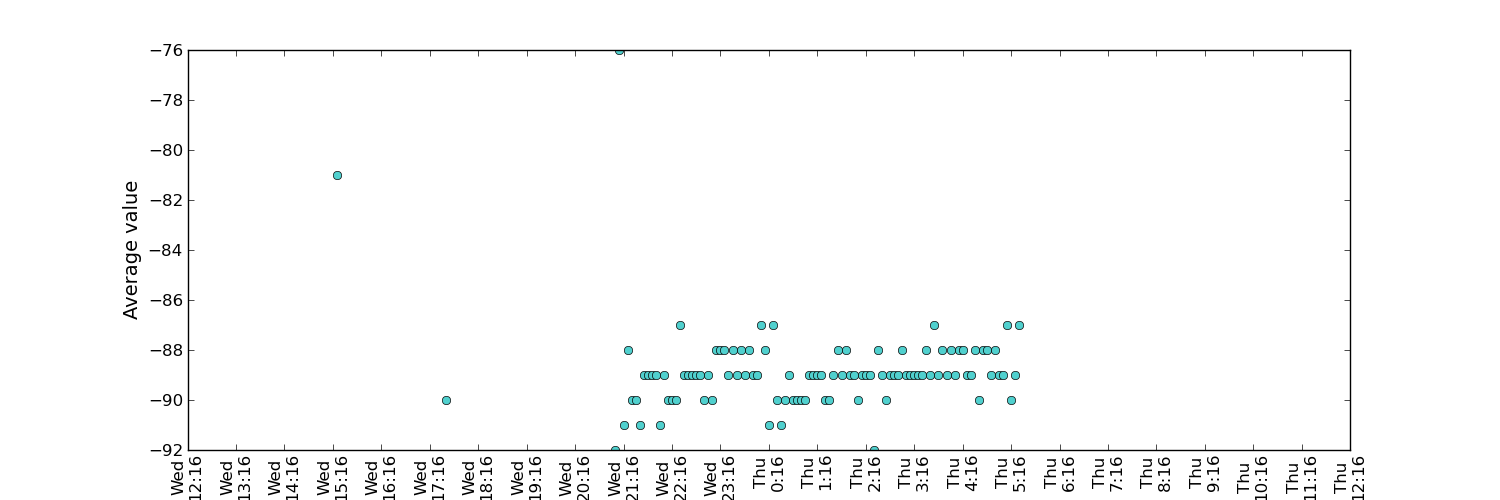
\includegraphics[width =\textwidth]{figures/combinations/user_6_sorted_1days_plot_3144_avg_sig.png}
\caption{Sample density of AP 3144}
\label{avg_6_2nd_day_3}
\end{figure}

\subsection{Running average signal strength}
\label{appendix_rn_avg}

This section contains the visualization for the running averages calculated for
$2$ (Fig.~\ref{user_1_AP1613_rn2avg_1d}), $5$
(Fig.~\ref{user_1_AP1613_rn2avg_1d}) and $10$
(Fig.~\ref{user_1_AP1613_rn2avg_1d}) minutes time bins for AP $1613$ identified
in a time frame of one day (Fig.\ref{user_1_APs_1d_ap}).

\begin{figure}[!h]
\centering
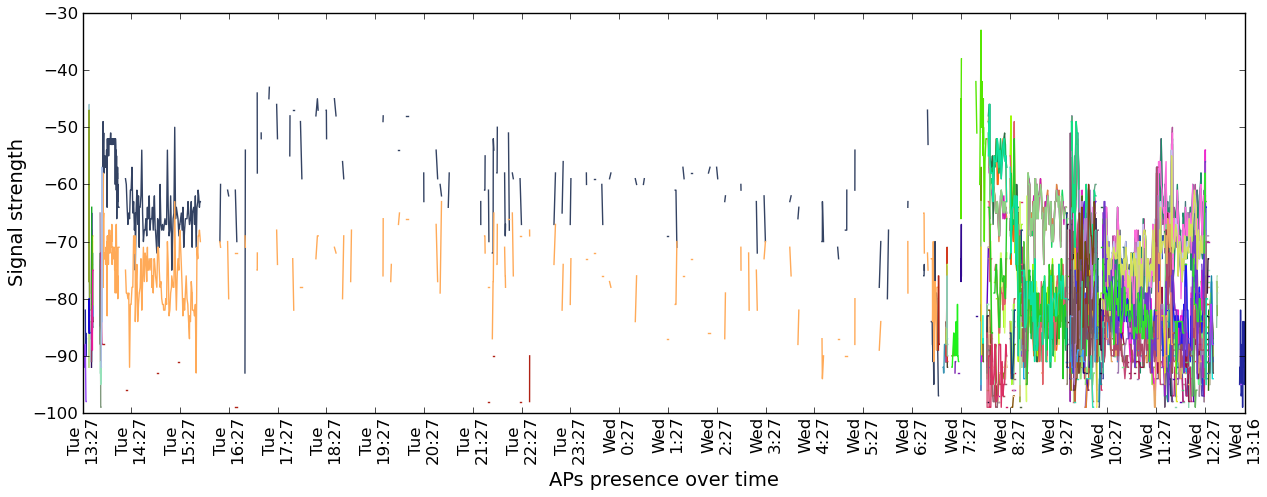
\includegraphics[width
=\textwidth]{figures/rn_avg/user_1_sorted_1days_plot.png}
\caption{Example of APs presence over time for userT}
\label{user_1_APs_1d_ap}
\end{figure}

\begin{figure}[!h]
\centering
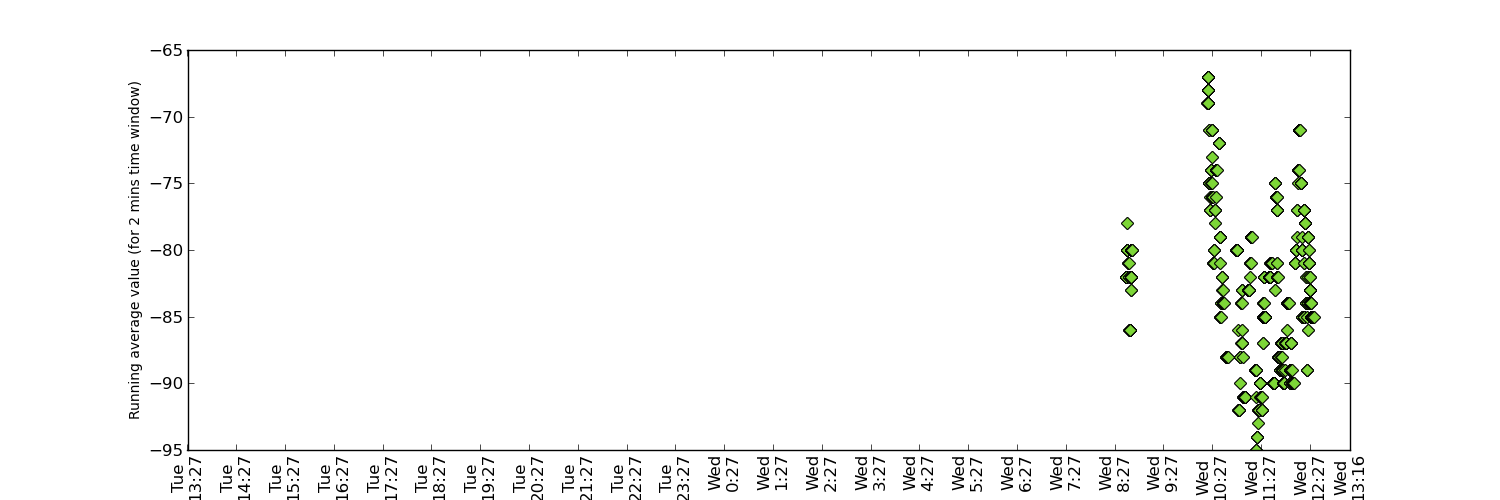
\includegraphics[width
=\textwidth]{figures/rn_avg/user_1_sorted_1days_plot_1613_rn_avg_sig_2.png}
\caption{Running average for AP 1613 for userT during 1 day (2 minute time
bins)}
\label{user_1_AP1613_rn2avg_1d}
\end{figure}

\begin{figure}[!h]
\centering
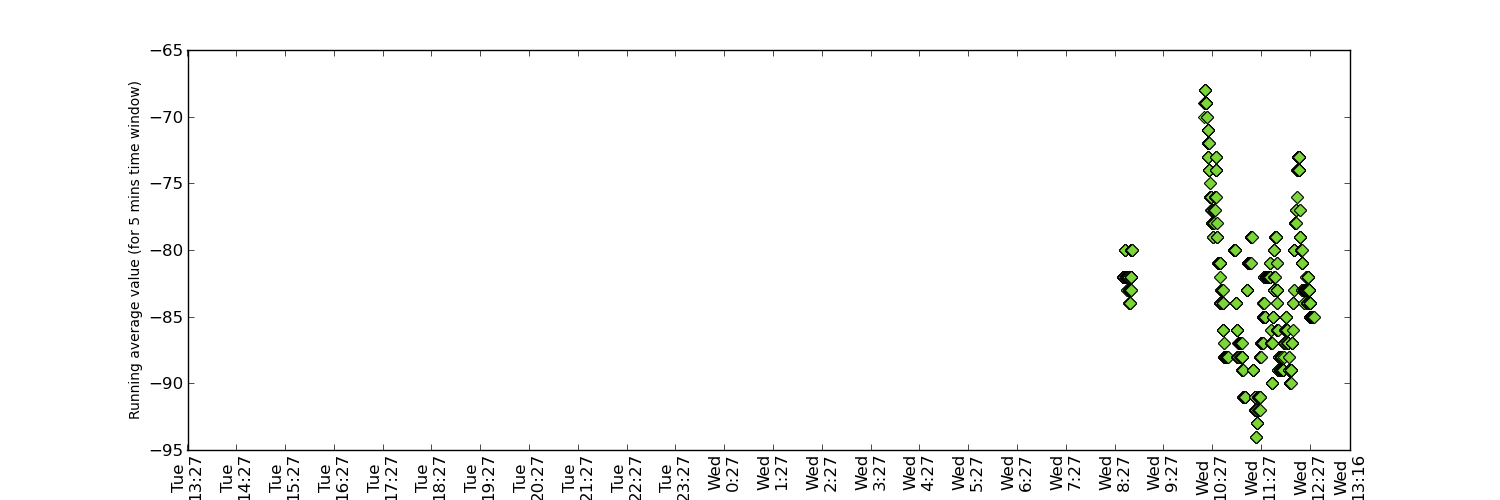
\includegraphics[width
=\textwidth]{figures/rn_avg/user_1_sorted_1days_plot_1613_rn_avg_sig_5.png}
\caption{Running average for AP 1613 for userT during 1 day (5 minute time
bins)}
\label{user_1_AP1613_rn5avg_1d}
\end{figure}

\begin{figure}[!h]
\centering
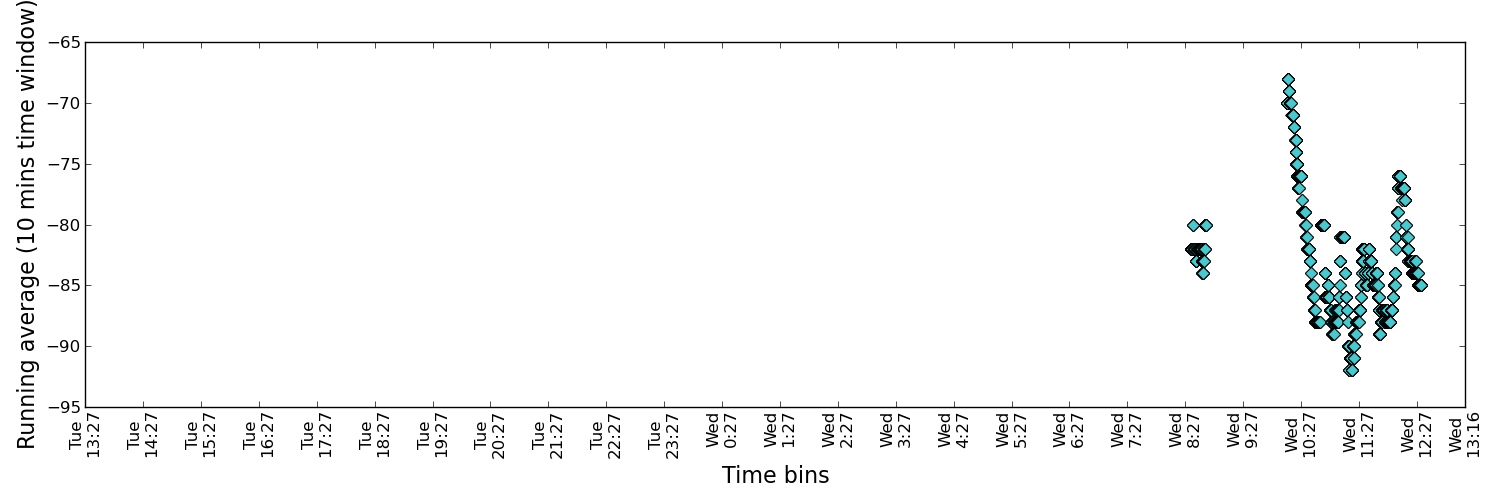
\includegraphics[width
=\textwidth]{figures/rn_avg/user_1_sorted_1days_plot_1613_rn_avg_sig_10.png}
\caption{Running average for AP 1613 for userT during 1 day (10 minute time
bins)}
\label{user_1_AP1613_rn10avg_1d}
\end{figure}

\subsection{Signal presence}